


\subsection{Factor Theory 因子理论}


\subsubsection{Factor theory}
\begin{itemize}
\item Factors are to assets what nutrients are to food.
    \begin{itemize}
    \item Factors matter, not assets.
        \begin{itemize}
        \item Need to look through asset class labels to understand the factor content.
        \end{itemize}
        
    \item Assets are bundles of factors.
        \begin{itemize}
        \item Risk premiums reflect their underlying factor risks.
        \end{itemize}
        
    \item Different investors need different risk factors.
        \begin{itemize}
        \item Different investors have different optimal exposures to different sets of risk factors.
        \end{itemize}
        
    \end{itemize}
\item Bad times: Each different factor defines a different set of bad times and the investors who bear these factor risks need to be compensated in equilibrium by earning factor risk premiums.
\item Risk premium: Investors are paid risk premiums in normal time as compensation for taking risks.
\item Exposure: Assets are bundles of factor risks, and it is the exposures to the underlying factor risks that earn risk premiums.
\end{itemize}
\begin{center}
    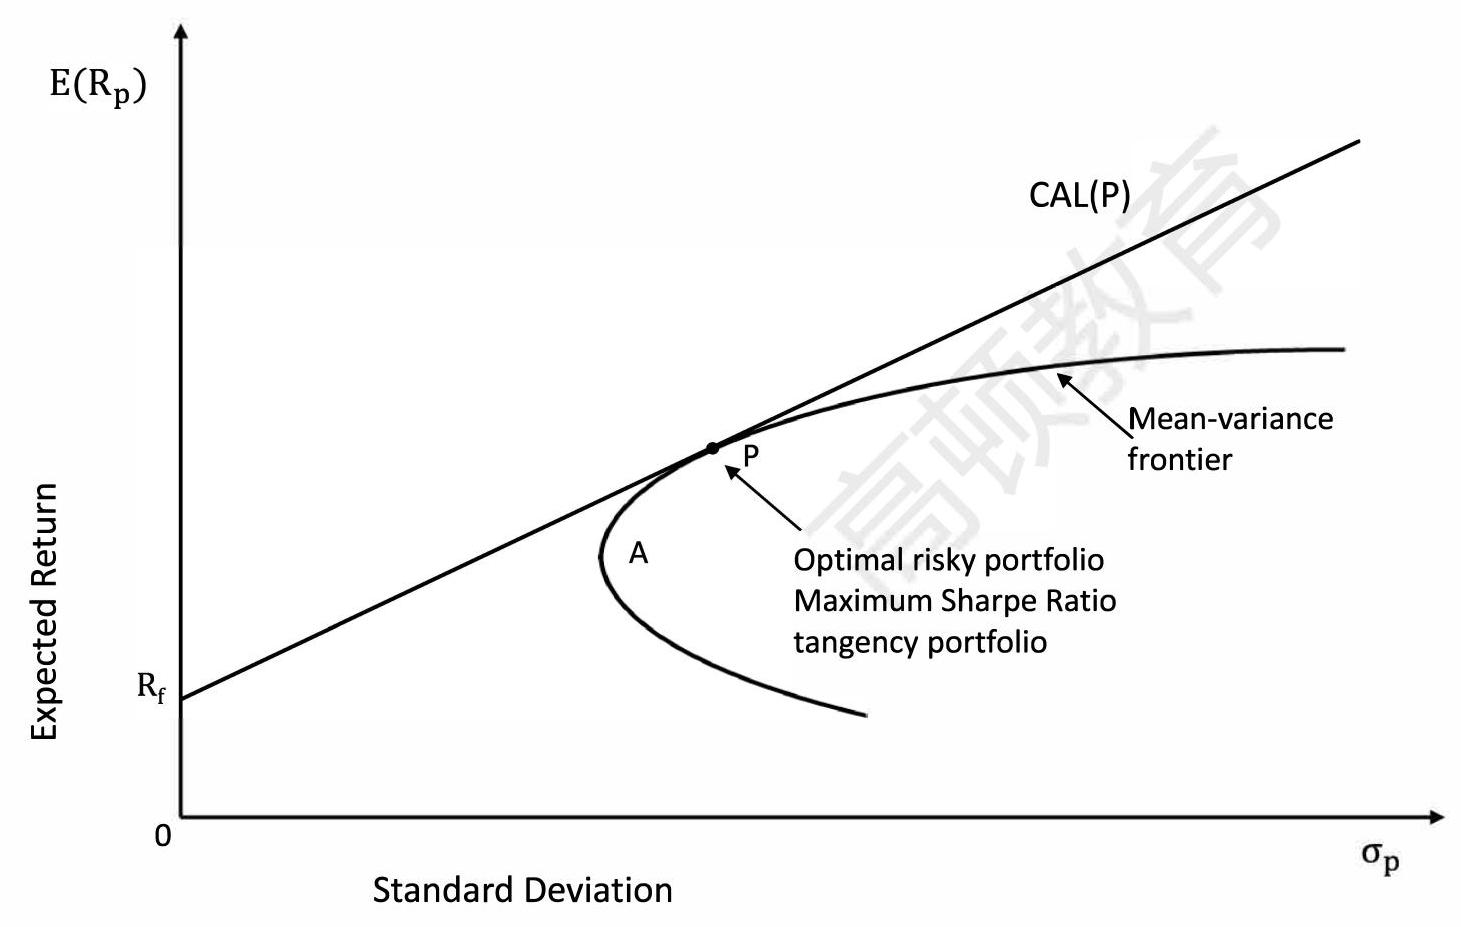
\includegraphics[width=0.9\textwidth]{images/StandardDeviation.jpg}
    \end{center}



\subsubsection{CAPM}
\begin{itemize}
\item An important theory of factor risk is the CAPM.
    \begin{itemize}
    \item One factor: market factor. All risky assets have risk premiums determined only by their exposure to the market portfolio.
 \[
E(R_i) = R_f + \beta (R_m - R_f)
\]
    \end{itemize}
\item Assumptions:
    \begin{itemize}
    \item Investors are expected to make decisions solely in terms of expected values and standard deviations of the returns on their portfolios.
    \item Investor plan for the same single holding period.
    \item Investor have homogeneous expectations or beliefs.
    \item An individual cannot affect the asset price by buying or selling action (price taker).
    \item All assets, including human capital, are tradable.
    \item Markets are frictionless, including no transaction cost and no taxes.
    \item All investments are infinitely divisible.
    \item Short sale is allowed unlimitedly.
    \item Unlimited lending and borrowing at the riskless rate.
    \end{itemize}
\item CAPM was revolutionary: the risk of an asset was not how the asset behaved in isolation but how that asset moved in relation( $\beta$ ) to other asset and to the market as a whole.

\item CAPM's one failure: the asset risk premiums depend only on the asset's beta and there is only one factor (market factor) matters.

\item Lesson 1: Factor - Don't hold an individual asset, hold the factor.
    \begin{itemize}
    \item Individual stocks: are exposed to the market factor, which carries the risk premium, but also have idiosyncratic risk, which is not rewarded by a risk premium.
    \item Market factor portfolio: investors can diversify away the idiosyncratic part and increase their returns.
    \item Systematic risk: The market factor is systematic and affects all assets.
    \end{itemize}
\item Lesson 2: Optimal exposure - Each investor has his or her own optimal exposure of factor risk
    \begin{itemize}
    \item Investors have different proportions of the risk-free asset
    and the market portfolio.
    \end{itemize}
\item Lesson 3: Risk premium - The factor risk premium is determined by risk aversion of average investor and the volatility of market.
\[
E(R_{\mathrm{m}}) - R_{f} = \bar{\gamma} \sigma_{m}^{2}
\]
    \begin{itemize}
    \item $\bar{\gamma}$ is the risk aversion of average investor: 100\% in the mean-variance efficient (MVE) portfolio position is the risk aversion of the market.
    \[
Utility = E(R) - \frac{1}{2} \gamma \sigma^{2}
\]
    \end{itemize}
\item Lesson 4: Beta - Risk is factor exposure
    \[ E(R) - R_f = \beta_i (E(R_m) - R_f) \]
    \[\beta_i = \left( \dfrac{cov(R_i, R_m)}{var(R_m)} \right) = \rho_{i,m} \dfrac{\sigma_i}{\sigma_m}\]
    
    
    \begin{itemize}
    \item The $\beta$ is a measure of how that stock co-moves with the market portfolio, and the higher the co-movement, the higher the asset's beta.
    \item Higher betas mean low diversification benefits.
    \item If the asset pays off when the market has losses, the asset has a low beta. If the payoff of an asset tends to be high in bad times, this is a valuable asset to hold and its risk premium is low.
    \end{itemize}
\end{itemize}



\subsubsection{Multifactor models}
\begin{itemize}
\item Multifactor models recognize the bad times can be defined more broadly than just bad returns on the market portfolio.
    \begin{itemize}
    \item In equilibrium, investors must be compensated for bearing these multiple sources of factor risk.
    \end{itemize}
    
\item Pricing kernel (stochastic discount factor, SDF)
    \begin{itemize}
    \item We denote the SDF as m which is an index of bad time. Any risk premium exists because it is compensation for losing money during bad times.
    \[ m = a + b_1 f_1 + b_2 f_2 + \cdots + b_k f_k \]
\[ E(R_i) - R_f = \left( \frac{\mathrm{cov}(R_i, m)}{\mathrm{var}(m)} \right) \left( - \frac{\mathrm{var}(m)}{E(m)} \right) \notag 
= \beta_{i,m} \lambda_m \]
    \item Multi-beta relation for an asset's premium:
    \[E(R_i) = R_f + \beta_{i,1} E(f_1) + \beta_{i,2} E(f_2) + \cdots + \beta_{i,k} E(f_k)\]
    \begin{center}
        
$E(f_k)$ is the risk premium of factor $k$.

$B_{ik}$ is the beta of asset $i$ with respect to factor $k$.
\end{center}

    \end{itemize}
    
\end{itemize}



\subsubsection{CAPM (Cont.)}
\begin{itemize}
\item Failures of the CAPM:
    \begin{itemize}
    \item CAPM assumes that investors have only financial wealth.
        \begin{itemize}
        \item Investors have unique income streams and liabilities.
        \end{itemize}
    \item Investors have mean-variance utility.
        \begin{itemize}
        \item Asymmetric treatment of risk (more distressed by losses than pleased by gains)
        \end{itemize}
    \item Single-period investment horizon.
    \item Investors have homogeneous expectations.
        \begin{itemize}
        \item In reality, investors do not all share the same beliefs.
        \end{itemize}
    \item No taxes or transaction costs.
    \item Individual investors are price takers.
        \begin{itemize}
        \item The informed investor is trading and moving prices.
        \end{itemize}
    \item Information is costless and available to all investors.
    \end{itemize}
    
\end{itemize}



\subsubsection{The fall of efficient market theory}
\begin{itemize}
\item There are three forms of efficient markets:
\begin{table}[htbp]
    \centering
    \begin{tabular}{@{}lp{8cm}@{}}
        \toprule
        Weak form & Asset prices fully reflect all market data. \\
        \midrule
        Semi-strong form & Asset prices reflect all publicly known and available information. \\
        \midrule
        Strong form & Asset prices fully \textbf{reflect all information}, which includes both public and private information. \\
        \bottomrule
    \end{tabular}
\end{table}
    \begin{itemize}
    \item Speculative trading is costly, active management is a loser's game and investors cannot beat the market
    \end{itemize}
\item Market near-efficiency (Sanford Grossman \& Joseph Stiglitz):
    \begin{itemize}
    \item Assume it is costly to collect information and to trade on that information
    \item Active managers earn excess returns as a reward for gathering and acting on costly information.
    \item Active managers search for pockets of inefficiency, and in doing so cause the market to be almost efficient.
    \end{itemize}
\item The deviations from efficiency have two forms:
    \begin{itemize}
    \item Rational explanation: high returns compensate for losses during bad times. The key is defining those bad times.
    \item Behavioral explanation:
        \begin{itemize}
        \item Under- or overreaction to news or events (inefficient updating of beliefs or ignoring some information).
        \item Structural barriers: e.g. entry of capital, regulatory requirements
        \end{itemize}
    \end{itemize}
\end{itemize}



\subsection{Factors}



\subsubsection{Types of factors}
\begin{itemize}
\item Assets are buffeted by risk factors. The risk factors offer premiums to compensate investors for bearing losses during bad times.
    \begin{itemize}
    \item Macro, fundamental-based factors
    \item Investment factors
        \begin{itemize}
        \item Static factors: simply go long to collect a risk premium ( e.g., market factors).
        \item Dynamic factors: can only be exploited through constantly trading different types of securities.
        \end{itemize}
    \end{itemize}
\end{itemize}



\subsubsection{Macro factors}
\begin{itemize}
\item Macro factors affect all investors and the prices of assets. Although macro factors may have different impact on different investors, in general, bad outcomes of macro factors define bad times for the average investor.
\item A shock to a factor matters more than the level of the factor.
    \begin{itemize}
    \item Economic growth
    
    \item Inflation
    \item Volatility
    \end{itemize}
\item Economic growth:


\begin{table}[htbp]
    \centering
    \caption{Asset Returns and Volatility in Different Economic Conditions}
    \begin{tabular}{l l c c c c c}
        \toprule
        &  & Large stocks & Small stocks & Govt. bonds & Invest. grade & High yield \\
        \midrule
        \multirow{2}{*}{Recession} 
        & Return & 5.6\% & 7.8\% & 12.3\% & 12.6\% & 7.4\% \\
        & volatility & 23.7\% & 33.8\% & 15.5\% & 16.6\% & 18.1\% \\
        \midrule
        \multirow{2}{*}{Expansion} 
        & Return & 12.4\% & 16.8\% & 5.9\% & 6.0\% & 7.7\% \\
        & volatility & 14\% & 21.2\% & 9.3\% & 7.8\% & 6.8\% \\
        \midrule
        \multicolumn{2}{l}{Average return} & 11.3\% & 15.3\% & 7\% & 7\% & 7.6\% \\
        \bottomrule
    \end{tabular}

    \footnotesize{NBER, 1952:Q1 to 2011:Q4 quarterly frequency}
\end{table}
    \begin{itemize}
    \item Volatility tends to be very high during bad times. All asset returns are much more volatile during recessions.
    \item Risky assets generally perform poorly and are much more volatile during periods of low economic growth.
    \end{itemize}


    \begin{table}[htbp]
        \centering
        \caption{Investor - Investment - Performance Relationship}
        \begin{tabular}{|c|c|c|}
            \hline
            Investor & Investment & Performance \\
            \hline
            Can weather recessions & More risky assets & Higher returns in long term to compensate losses during recession \\
            \hline
            Cannot weather recessions & Less risky assets & \textcolor{blue}{Lower returns in long term due to better performance in recession} \\
            \hline
        \end{tabular}
    \end{table}


        \footnotesize{Price for low exposure to growth risk}
\item Inflation:

\begin{table}[htbp]
    \centering
    \begin{tabular}{l l c c c c c}
        \toprule
        &  & Large stocks & Small stocks & Govt. bonds & Investment grade & High yield \\
        \midrule
        \multirow{2}{*}{Inflation} 
        & Low & 14.7\% & 17.6\% & 8.6\% & 8.8\% & 9.2\% \\
        & High & 8\% & 13\% & 5.4\% & 5.3\% & 6\% \\
        \midrule
        \multicolumn{2}{l}{Average return} & 11.3\% & 15.3\% & 7\% & 7\% & 7.6\% \\
        \bottomrule
    \end{tabular}
    \begin{itemize}
        \item \checkmark High inflation tends to be bad for both stocks and bonds.
    \end{itemize}
\end{table}

\item Volatility:


\begin{table}[htbp]
    \centering
    \begin{tabular}{lccc}
        \toprule
         & VIX changes & Stock returns & Bond returns \\
        \midrule
        VIX changes & 1 & --.39 &.12 \\
        Stock returns & --.39 & 1 & --.01 \\
        Bond returns &.12 & --.01 & 1 \\
        \bottomrule
    \end{tabular}
\end{table}

    \begin{itemize}
    \item Volatility and stock returns: negative relations (leverage effect).
    \item Bonds offer some respite during periods of high volatility.
    \item Volatility is negatively linked to the returns of many assets
    and strategies.
    \item Volatility is a factor with a negative price of risk
        \begin{itemize}
            \item To collect a volatility premium requires selling volatility protection.
        \end{itemize}
    
    \end{itemize}
    
\item Manage volatility:
    \begin{itemize}
    \item Dislike volatility:
        \begin{itemize}
        \item Investors who is sensitive to volatility could increase bond position (but not always pay off in high volatility).
        \item Buy volatility protection (long put, volatility swap)
        \end{itemize}
    \item Can afford volatility: sell volatility protection (short put)
        \begin{itemize}
        \item Sell volatility generates high and steady payoffs during stable times which compensate large losses in a huge crash (inevitable large losses that occur every decade).
        \end{itemize}
    \end{itemize}
    

    
    \begin{center}
        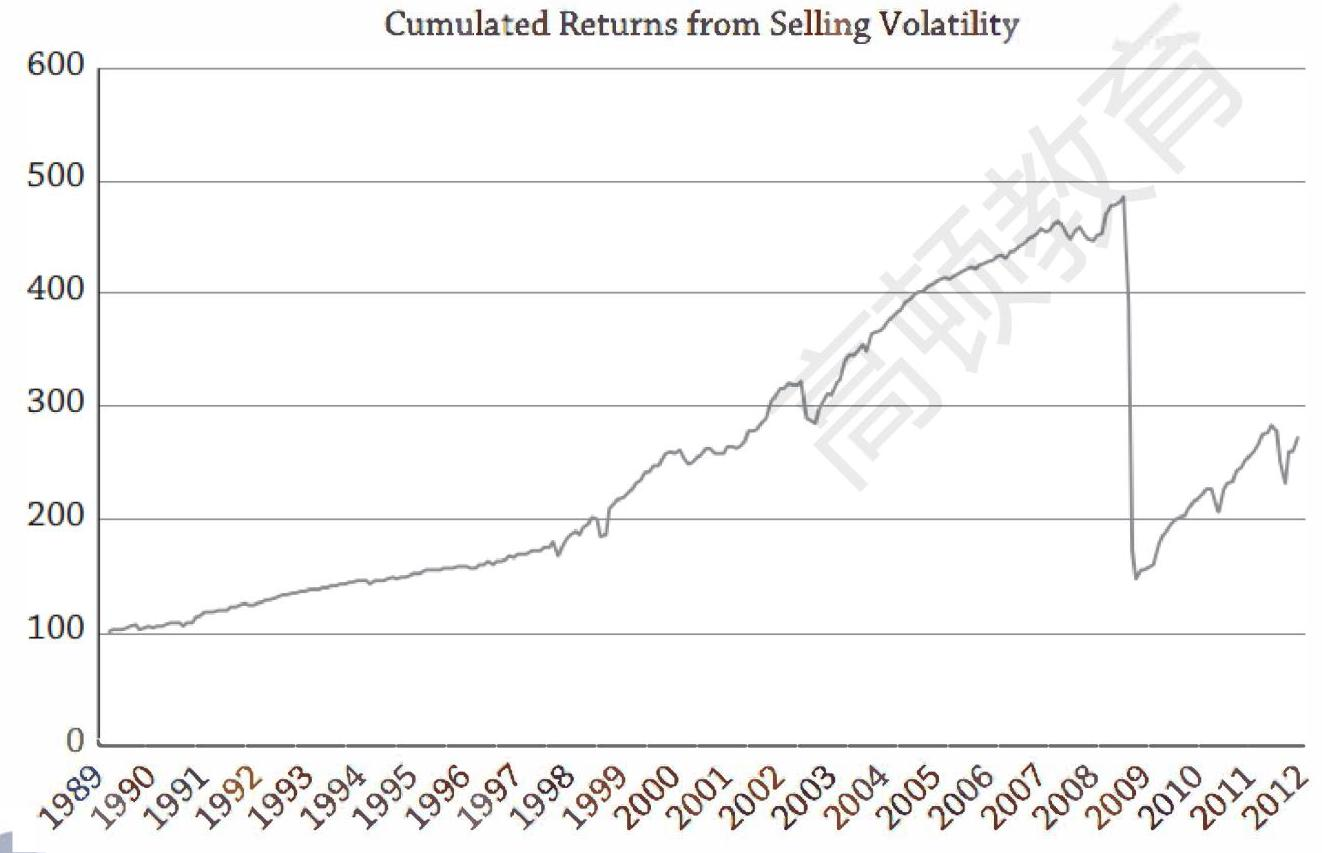
\includegraphics[width=0.9\textwidth]{images/Managevolatility.jpg}
        \end{center}

\item Other macro factors:
    \begin{itemize}
    \item Productivity risk
    \item Demographic risk
    \item Political risk
    \end{itemize}
\end{itemize}



\subsubsection{Dynamic factors}
\begin{itemize}
\item Macro factors like inflation and economic growth cannot be directly traded.
\item Dynamic factors have a big advantage that they can be easily traded in investors' portfolios ➔ long-short portfolio

    \begin{itemize}
    \item Style factors, investment factors, dynamic factors
    \item Smart beta, alternative beta
    \item Long-short factor
    \end{itemize}

    
 
    \begin{center}
        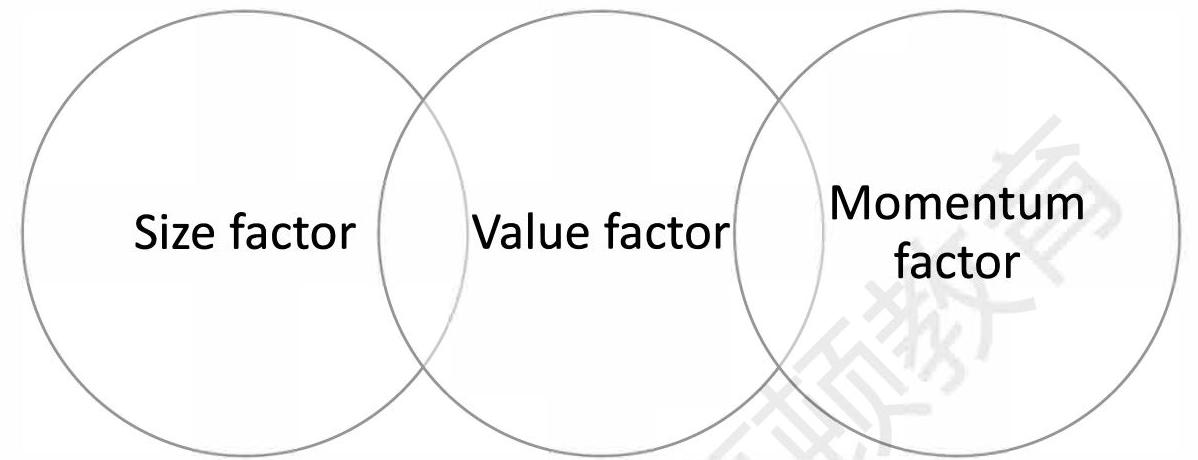
\includegraphics[width=0.9\textwidth]{images/Dynamic factors.jpg}
        \end{center}
\item Fama-French three-factor model: incorporates the systematic factors of market index, firm size (market capitalization) and book-to-market ratio:
\[
E(R_i) = R_f + \beta_{i,MKT} E(R_m - R_f) +  \beta_{i,SMB} E(SMB) + \beta_{i,HML} E(HML)
\]
\end{itemize}



\subsubsection{Size factors}
\begin{itemize}
\item Size factor: The SMB factor was designed to capture the outperformance of small firms relative to large firms.
    \begin{itemize}
    \item Since the mid-1980s there has not been any significant size effect.
    \item Responses to the disappearance of the size effect: 
        \begin{itemize}
        \item The original discovery of the size premium could have just been data mining.
        \item Rational investors bid up the price of small cap stocks until the effect was removed.
        \end{itemize}
    \end{itemize}
    
\end{itemize}



\subsubsection{Value factors}
\begin{itemize}
\item Value investing: Long value stocks and short growth stocks.
    \begin{itemize}
    \item Growth stocks: low book-to-market ratios
    \item Value stocks: high book-to-market ratios
    \end{itemize}

\item Rational theories of the value premium
    \begin{itemize}
    \item Flexibility of response to shock: value firms and growth firms differ in how flexible they are and how quickly they can respond to shocks.
    \item Value firms are riskier because they cannot shift their firm activities to more profitable activities in bad times (high and asymmetric adjustment costs).
    \end{itemize}

\item Behavioral theories of the value premium
    \begin{itemize}
    \item Overreaction or overextrapolation: investors tend to overextrapolate past growth rates into the future.
        \begin{itemize}
        \item Value stocks are cheap because investors underestimate their growth prospects.
        \item Growth firms are expensive because investors overestimate their growth prospects.
        \end{itemize}
    \end{itemize}
\end{itemize}

\subsubsection{Momentum factors}
\begin{itemize}
\item Momentum strategy: is to buy stocks that have gone up over the past six (or so) months (winners) and short stocks with the lowest returns over the same period (loser). Momentum is also called "trend" investing.
    \begin{itemize}
    \item Momentum effect: winner stocks continue to win and losers continue to lose.
    \end{itemize}

\item Four-factor model (Carhart model):
\[
E(R_i) = R_f + \beta_{i,MKT} E(R_m - R_f) + \beta_{i,SMB} E(SMB) + \beta_{i,HML} E(HML) + \beta_{i,WML} E(WML)
\]
\begin{center}
    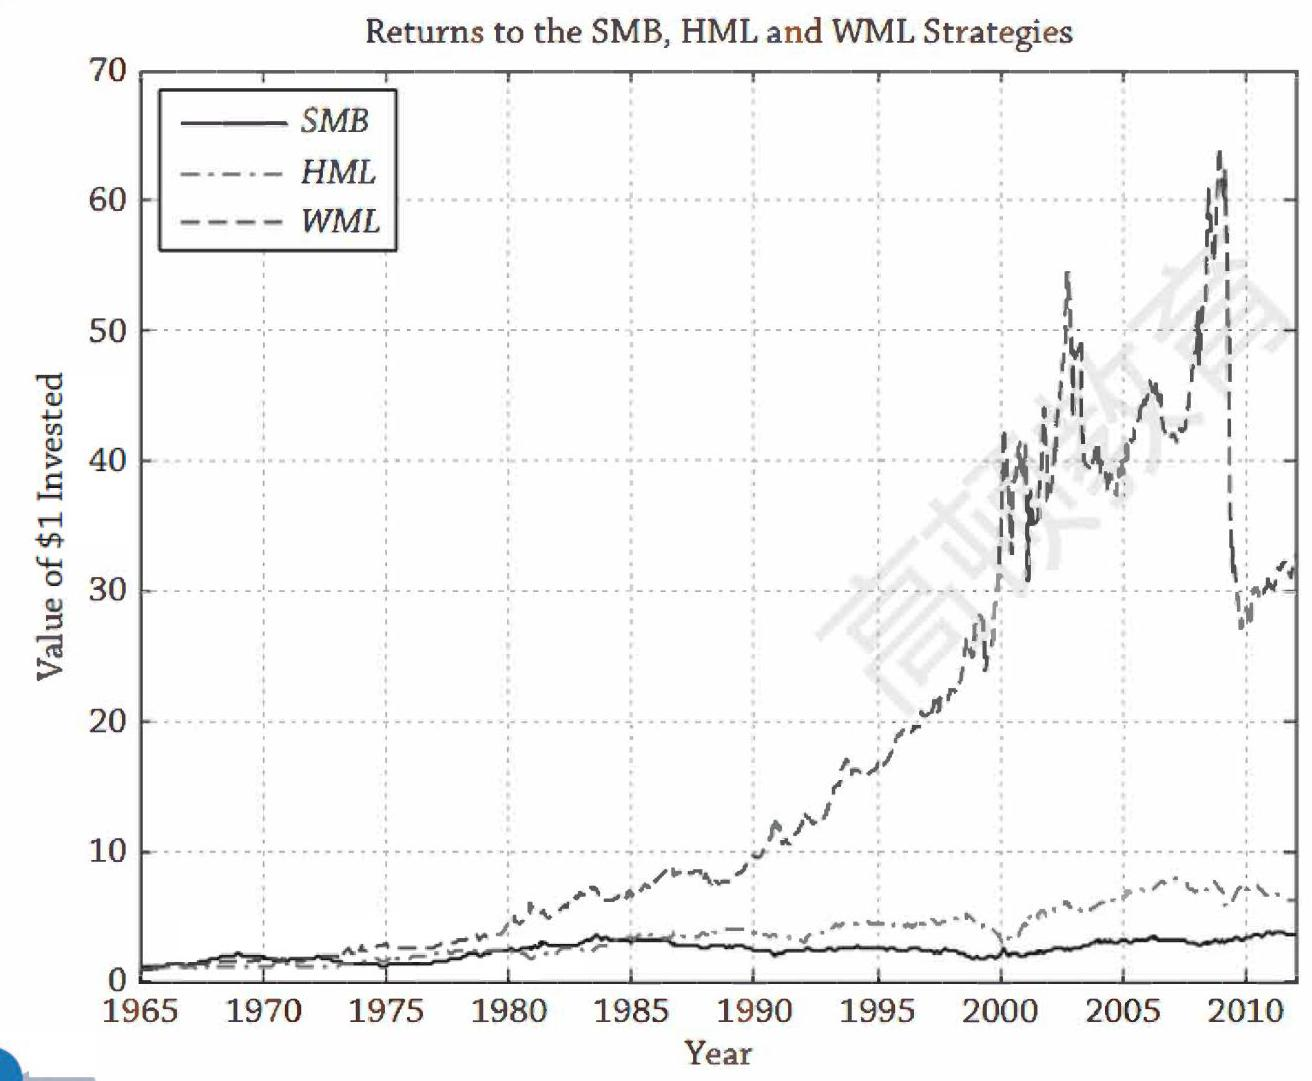
\includegraphics[width=0.9\textwidth]{images/Returns to the SMB.jpg}
    \end{center}
\item Characterizing momentum risk:
    \begin{itemize}
    \item Monetary policy and government risk during extraordinary times: for the loser stocks, government bailouts put a floor underneath the prices of these stocks to stop the tendency to keep losing.
    \end{itemize}
\item Behavioral theories of the momentum premium: momentum can be generated in two ways
    \begin{itemize}
    \item Delayed overreaction: causes the price to persistently drift upward
    \item Underreaction: the price does not go up as much as it should have to fully reflect how good the news actually was. Investors then learn and cause the stock to go up again the next period.
    \end{itemize}
        
\end{itemize}
    



\subsubsection{Summaries about dynamic factors}
\begin{itemize}
\item The size, value and momentum strategies are all crosssectional strategy, meaning that it compares one group of stocks against another group of stocks in the cross section.
    \begin{itemize}
    \item Momentum strategy: positive feedback strategy. Stocks with high past returns are attractive, momentum investors continue buying them and they continue to go up.
    \item Value strategy: negative feedback strategy. Stocks with declining prices eventually fall far enough that they become value stocks.
    \end{itemize}

    \begin{center}
        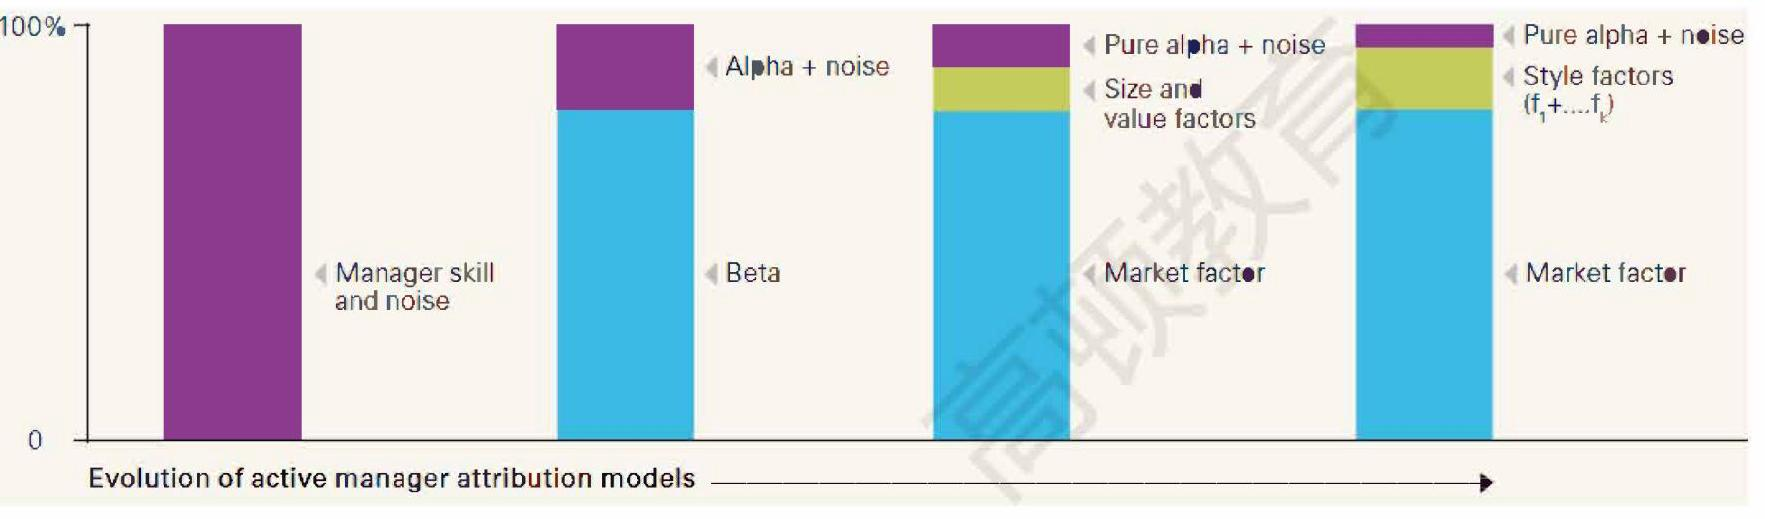
\includegraphics[width=0.9\textwidth]{images/0196d85e-4a46-766d-a7d3-d988c51d451d_62_2_399_1765_519_0.jpg}
        \end{center}

        \begin{center}
            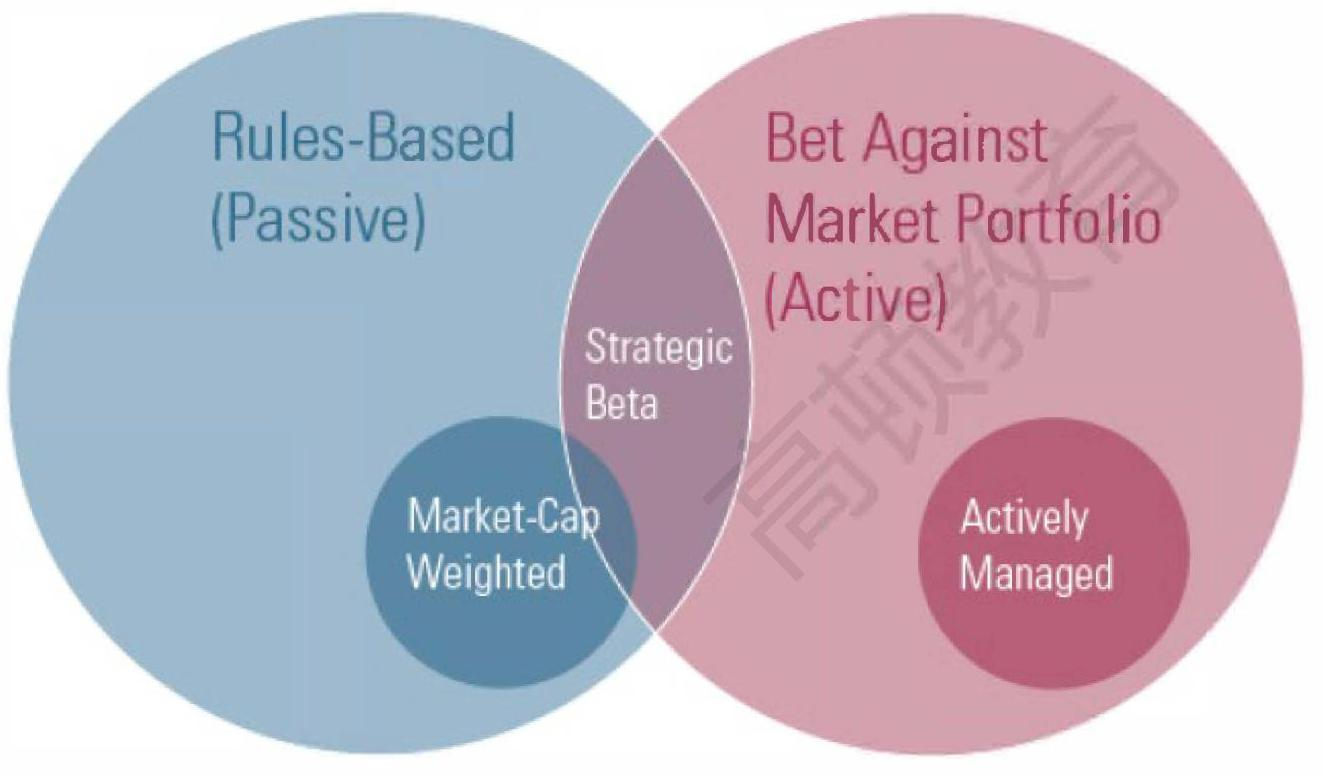
\includegraphics[width=0.9\textwidth]{images/Source Blackrock.jpg}
            \end{center}
            \begin{center}
                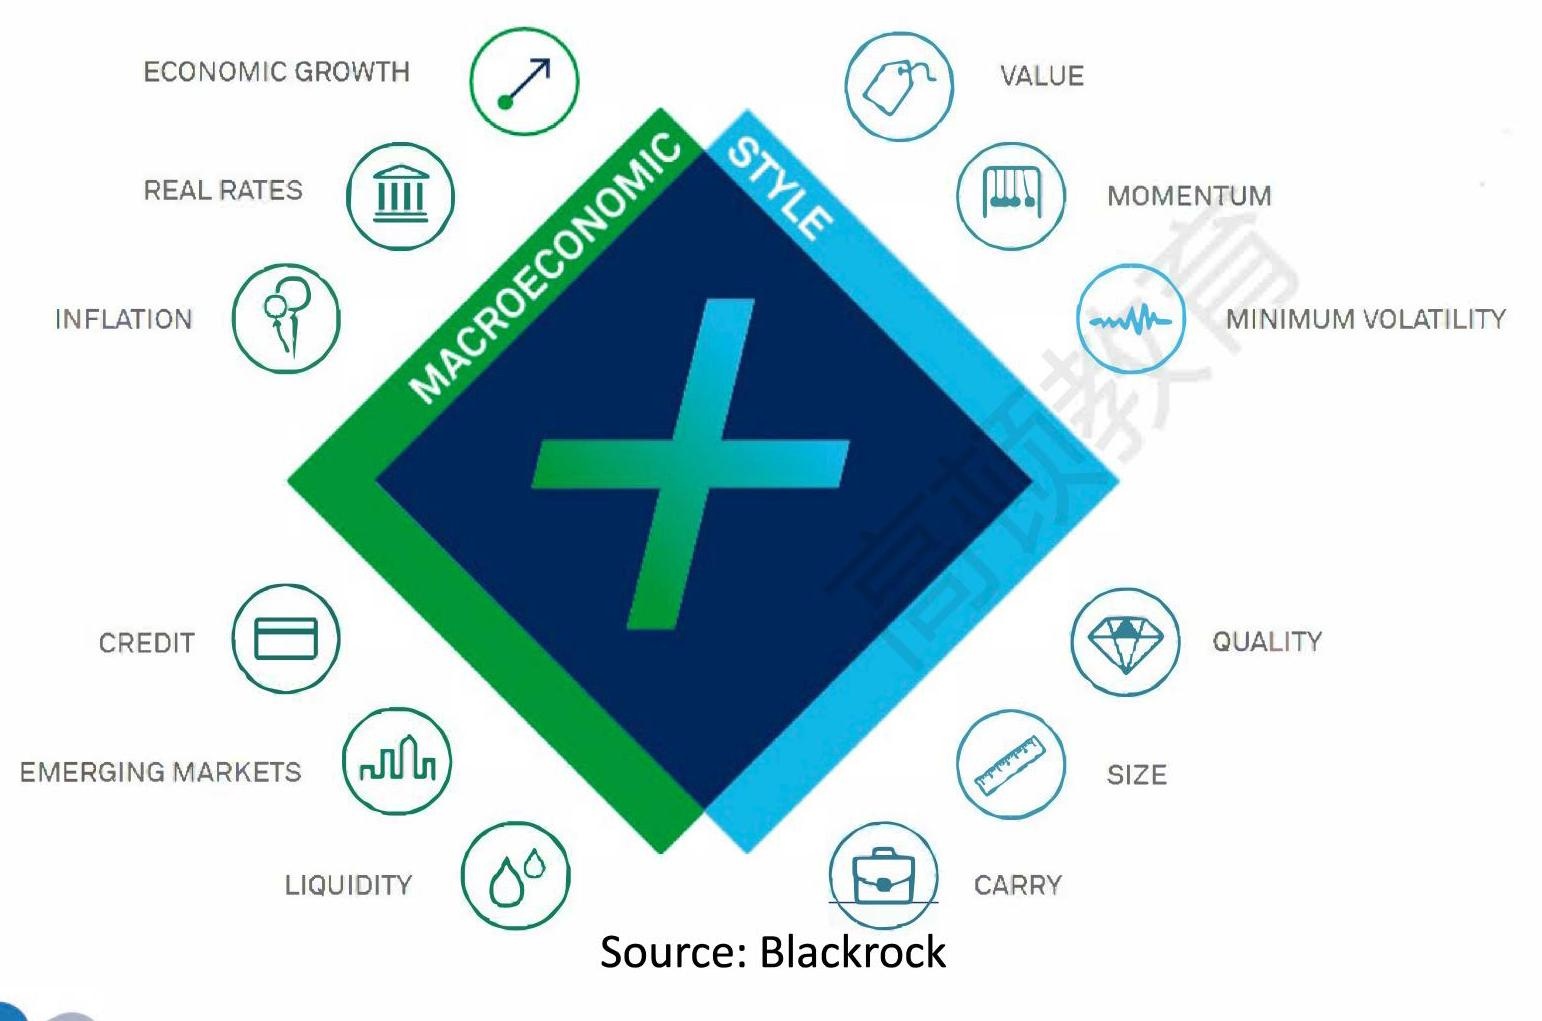
\includegraphics[width=0.9\textwidth]{images/0196d85e-4a46-766d-a7d3-d988c51d451d_64_100_231_1542_1021_0.jpg}
                \end{center}
            
                \begin{center}
                    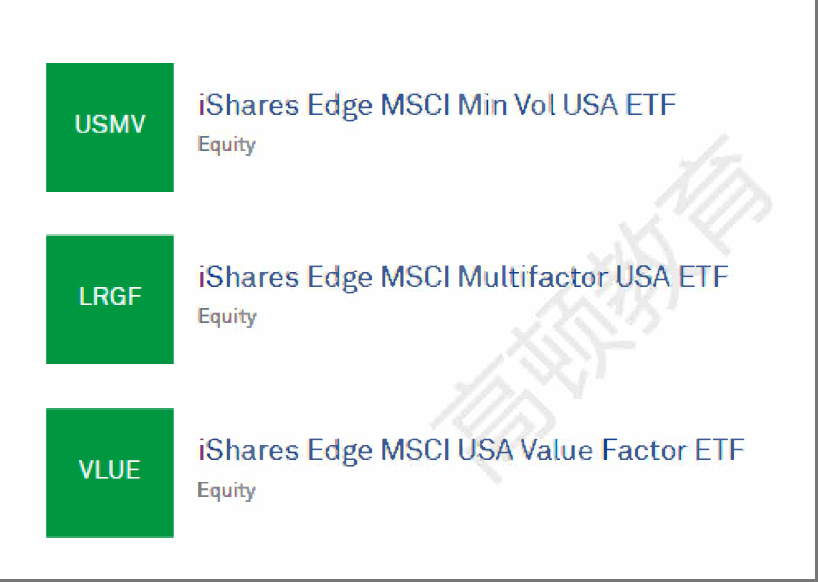
\includegraphics[width=0.9\textwidth]{images/111.png}
                    \end{center} 
                    
                    \begin{center}
                        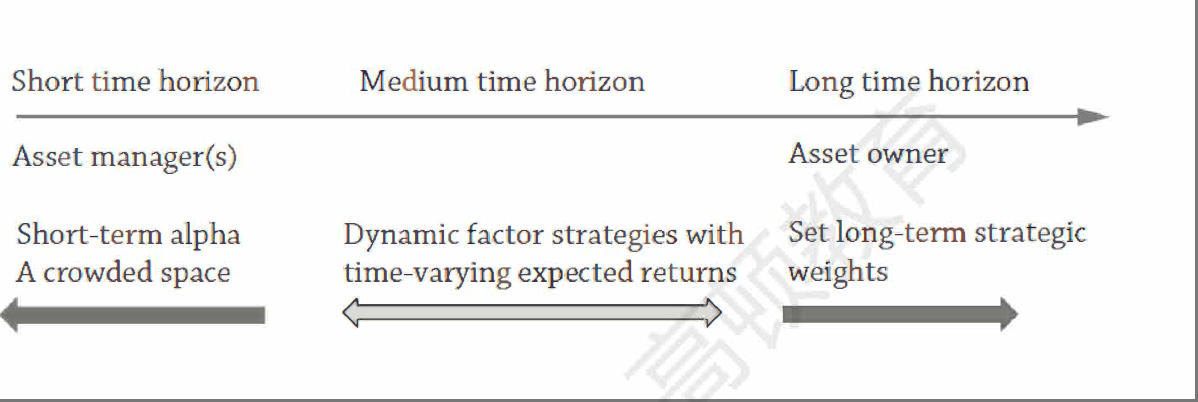
\includegraphics[width=0.9\textwidth]{images/222.jpg}
                        \end{center}
                        \begin{center}
                            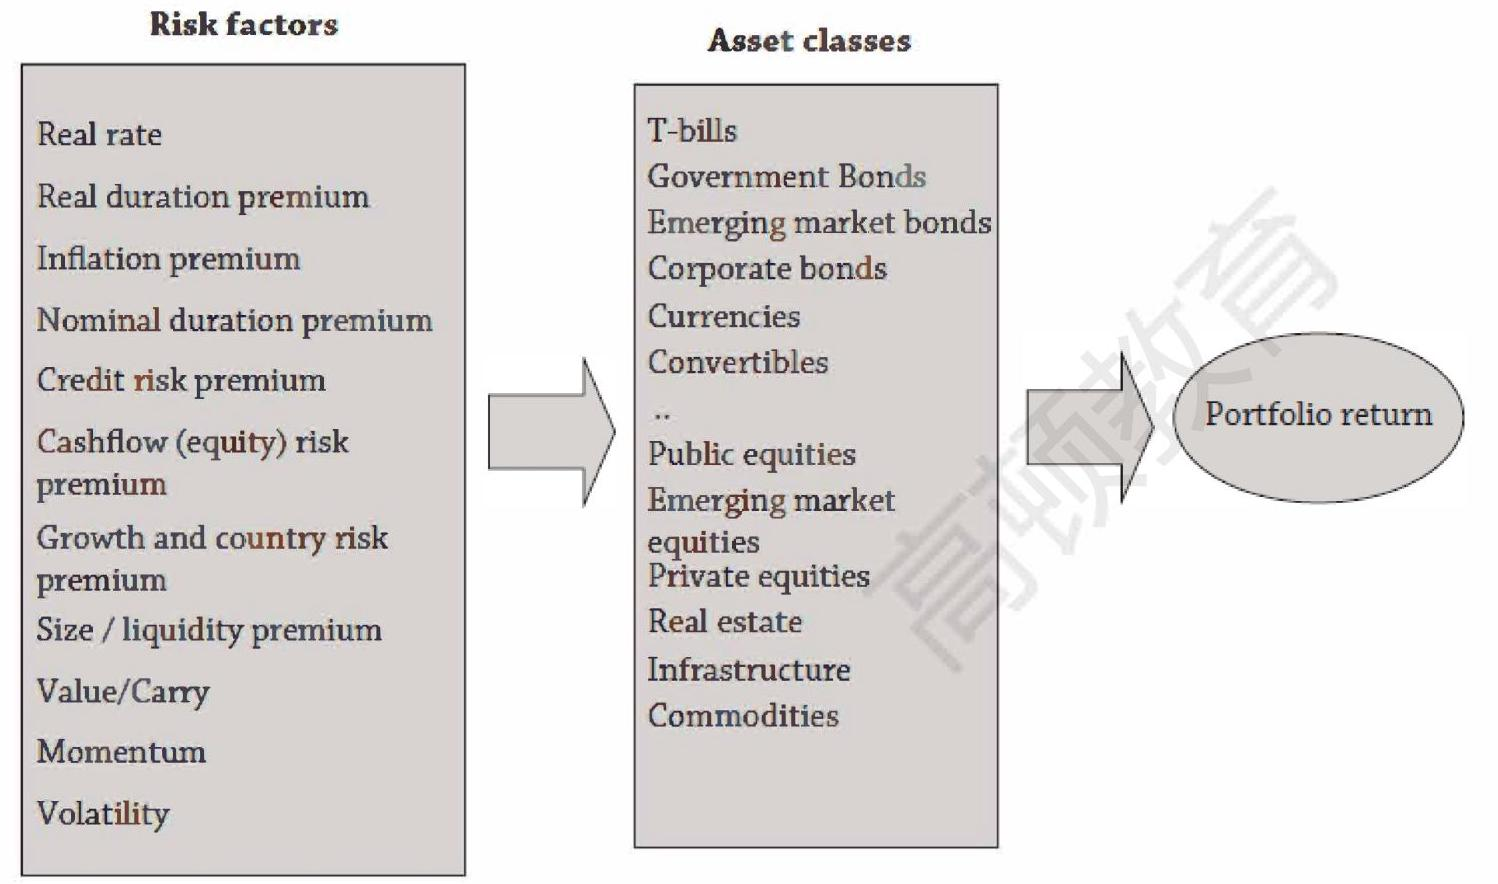
\includegraphics[width=0.9\textwidth]{images/0196d85e-4a46-766d-a7d3-d988c51d451d_67_61_229_1498_884_0.jpg}
                            \end{center}
\end{itemize}


\subsection{Alpha (and the Low-Risk Anomaly)}


\subsubsection{Active management}
\begin{itemize}
\item Alpha: average return in excess of a benchmark. Benchmark is passive and can be produced without any particular investment knowledge or even human intervention.
    \begin{itemize}
    \item Excess return (active returns): \( r_t^{ex} = r_t - r_t^{bmk} \)

    \item Average excess return:
    \(
    \alpha = \frac{1}{T} \sum_{t = 1}^{T} r_t^{ex}
    \)
    \item (where there are T observations in the sample)
    \end{itemize}
\item \(\text{Tracking error} = \bar{\sigma} = \text{stdev}(r_t^{ex})\)
    \begin{itemize}
    \item Tracking error constraints are imposed to ensure a manager does not stray too far from the benchmark. The larger the tracking error, the more freedom the manager has.
    \end{itemize}

\item Information ratio: the average excess return per unit of risk.
\[
\text{IR} = \frac{\text{active return}}{\text{tracking error}} = \frac{\alpha}{\bar{\sigma}}
\]
    \begin{itemize}
    \item Special case: when the benchmark is risk-free rate
    \[
\alpha = \overline{r_t - r_{ft}}
\]
\[
\text{IR} = \text{Sharpe Ratio} = \frac{\overline{r_t - r_{ft}}}{\sigma}
\]

    \end{itemize}
\item Grinold fundamental law:
\[
\text{IR} \approx \text{IC} \times \sqrt{\text{BR}}
\]
    \begin{itemize}
    \item Information coefficient (IC): the correlation of the manager's forecast with the actual returns
    \item The breadth of the strategy (BR): how many bets are taken
    \end{itemize}
\item Creating alpha: by making bets that deviate from that benchmark. The key to generating alpha is forecasting.
    \begin{itemize}
    \item How good asset managers at forecasting
    \item  How many bets
    \end{itemize}
\item Assumptions of fundamental law: each active return is independent from the other active return forecasts for that period and independent from the forecast for that security in subsequent periods.

\item Limitations of fundamental law :
    \begin{itemize}
    \item ICs are assumed to be constant across BR.
    \item Manager whom you find may truly have a high IC, but the one hundredth manager whom you hire probably does not.
    \item It is difficult to have truly independent forecasts in BR.
    \end{itemize}
\end{itemize}



\subsubsection{Benchmarks}
\begin{itemize}
\item Ideal benchmark:
    \begin{itemize}
    \item Well defined
    \item Tradable
    \item Replicable
    \item Adjusted for risk
    \end{itemize}
\item Index benchmark

\begin{align}
    r_t - r_{ft} &= 0.0344 + 0.7272 \times (r_{\mathrm{t}}^{R1000} - r_{ft}) + \varepsilon_t \\
    r_t &= \colorbox{red!20}{0.0344} + \colorbox{red!20}{0.2728$r_{ft}$ + 0.7272$r_{\mathrm{t}}^{R1000}$} + \varepsilon_t \\
    &\quad \underset{\alpha}{\downarrow} \quad \quad \quad \quad \quad \quad \quad \quad \underset{r_{\mathrm{bmk}}}{\downarrow} \notag
    \end{align}
    \begin{itemize}
        \item \textcolor{blue}{\checkmark} The benchmark portfolio holding 27\% in the risk - free asset and 73\% in the Russell 100
        \item \textcolor{blue}{\checkmark} Naïve benchmark
    \end{itemize}
    \begin{align}
    r_t &= \colorbox{red!20}{0.015} + \colorbox{red!20}{$r_{\mathrm{t}}^{R1000}$} + \varepsilon_t \\
    &\quad \underset{\alpha}{\downarrow} \quad \quad \quad \quad \underset{r_{\mathrm{bmk}}}{\downarrow} \notag
    \end{align}

\item Factor benchmarks are a combination of factors
    \begin{itemize}
    \item The factor benchmark describes the systematic components of asset i's return.
    \[
E(r_i) - r_f = \beta_i [E(r_m) - r_f]
\]
\[
\text{if } \beta_i = 1.3 \rightarrow E(r_i) = -0.3r_f + 1.3E(r_m)
\]
\[
E(r_i) = \alpha_{\mathrm{i}} + \colorbox{red!20}{$[-0.3r_f + 1.3E(r_m)]$} \newline \underset{E(r_{\mathrm{bmk}})}{\downarrow}
\]
    \end{itemize}

\item Factor regressions
\[
r_{\mathrm{it}} - r_{ft} = \alpha + \beta (r_{\mathrm{mt}} - r_{ft}) + s SMB_t + h HML_t + u UMD_t + \varepsilon_{it}
\]
\begin{itemize}
    \item \(\mathbf{s = 0}\) if a stock co - moves neither with small nor large stocks, it's a medium - size stock
    \item \(\mathbf{s > 0}\) stock moves together with small stocks
    \item \(\mathbf{s < 0}\) stock moves together with large stocks
\end{itemize}


\begin{table}[htbp]
    \centering
    \begin{tabular}{l l c}
        \toprule
         & Coefficient & T - stat \\
        \midrule
        Alpha & 0.68\% & 2.05 \\
        MKT loading & 0.66 & 8.26 \\
        SMB loading & -0.5 (large stock exposure) & -4.86 \\
        HML loading & 0.36 (value orientation) & 3.33 \\
        UMD loading & -0.04 & -0.66 \\
        Adj R$^2$ & 0.27 &  \\
        \bottomrule
    \end{tabular}
\end{table}

    \begin{itemize}
    \item Statistical significance of alpha: determines whether the alpha reliably indicates ability.
        \begin{itemize}
        \item Null ($H_0$): Alpha is zero
        \item Alternative (HA): Alpha is not zero
        \[
t(\hat{\alpha}) = \frac{\hat{\alpha} - 0}{\hat{\sigma}(e)/\sqrt{N}}
\]

        \end{itemize}
        
    \end{itemize}
    

\item Time-varying factor: introduced "style analysis" to handle time-varying benchmarks where the factor exposures evolve through time.
    \begin{itemize}
    \item Style analysis seeks to rectify two potential shortcomings of factor regression:
        \begin{itemize}
        \item The Fama-French portfolios are not tradable.
        \item The factor loadings may vary over time.
        \end{itemize}
    \item The collection of index funds that replicate the fund is called the "style weight."
    \end{itemize}
    
\item Time-varying factor
    \begin{itemize}
    \item Example: Style analysis with no shorting - Berkshire Hathaway Inc. (data from Jan. 2001 to December 2011)
    \end{itemize}

    \[
\begin{split}
r_{t + 1} &= \alpha_t + \beta_{SPY,t} SPY_{t + 1} \\
& \quad + \beta_{SPYV,t} SPYV_{t + 1} \\
& \quad + \beta_{SPYG,t} SPYG_{t + 1} + \varepsilon_{t + 1}
\end{split}
\]
\begin{itemize}
    \item $\alpha_t$
    \item $\beta_{SPY,t} SPY_{t + 1}$: SPY: SPDR S\&P 500 ETF, which is designed to mimic the S\&P 500.
    \item $\beta_{SPYV,t} SPYV_{t + 1}$: SPYV: SPDR S\&P 500 Value ETF, which tracks the S\&P 500 value index.
    \item $\beta_{SPYG,t} SPYG_{t + 1}$: SPYG: SPDR S\&P 500 Growth ETF, which replicates the S\&P 500 growth index.
    \item $\varepsilon_{t + 1}$
\end{itemize}
    \begin{itemize}
    \item Time-varying factor
        \begin{itemize}
        \item Style analysis with no shorting
        \end{itemize}
        \begin{center}
            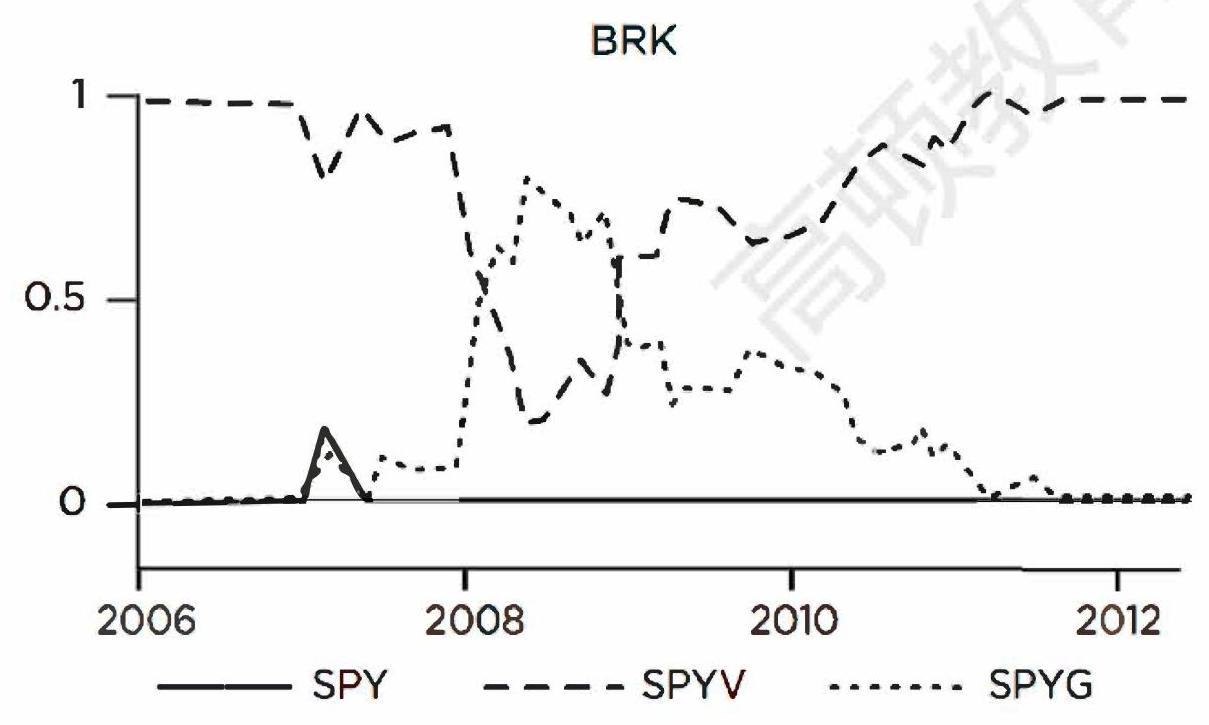
\includegraphics[width=0.9\textwidth]{images/101.jpg}
            \end{center}                  
              \begin{center}
                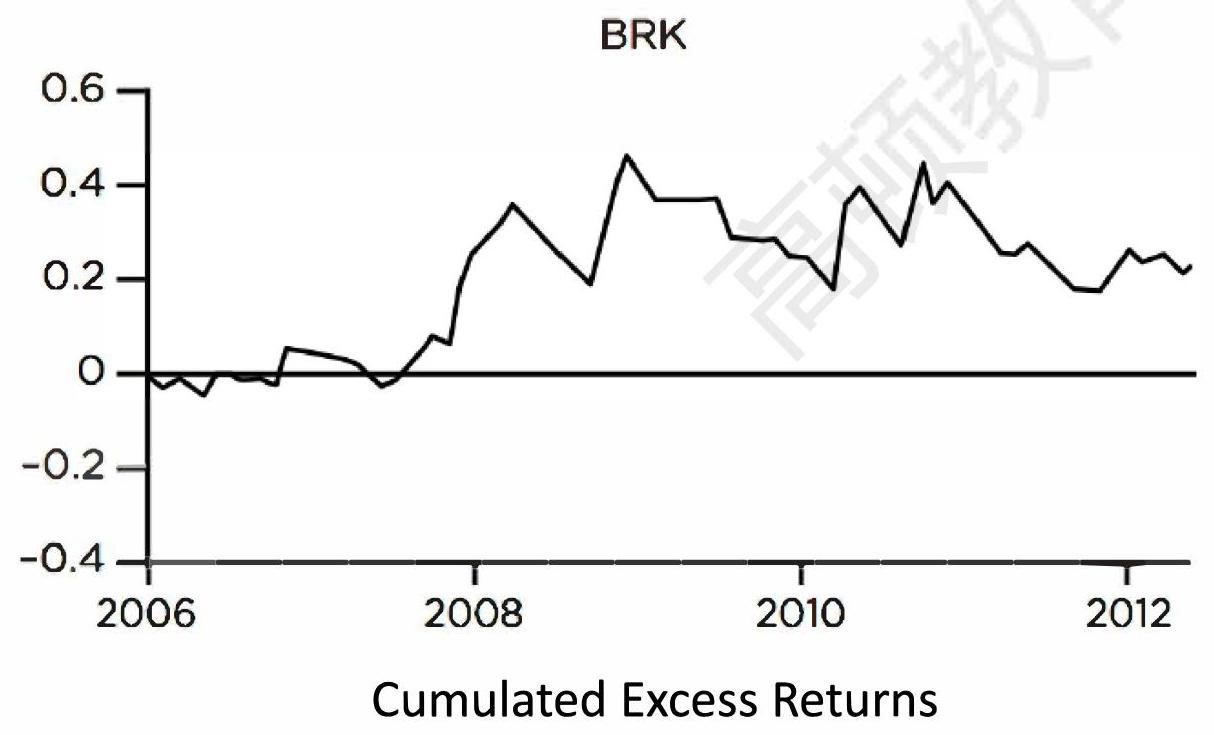
\includegraphics[width=0.9\textwidth]{images/202.jpg}
                \end{center} 
    \end{itemize}

\item Non-linear payoffs: alphas are computed in a linear framework. There are many nonlinear strategies, especially those involving dynamic option strategies, that can masquerade as alpha.
\item Why do dynamic, nonlinear strategies yield false measures of alpha?
    \begin{itemize}
    \item Buying and selling options changes the distribution of returns.
    \end{itemize}
    
\end{itemize}



\subsubsection{Low-risk anomaly}
\begin{itemize}
\item Traditional financial theory: in CAPM for example, there should be a positive relation between risk and return.

    
\item The risk anomaly: stocks with low betas and low volatilities have high returns.
    \begin{itemize}
    \item Volatility is negatively related to future returns.
    \item Realized beta is negatively related to future returns.
    \item Minimum variance portfolios do better than the market.
    \end{itemize}
    
    
\item Explanation:
    \begin{itemize}
    \item Leverage constraints: investors wish to take on more risk but are unable to take on more leverage.
    \item Agency problems: Institutional managers have constraints.
        \begin{itemize}
        \item Long only: If a stock has negative alpha, manager needs to short stock and he or she cannot do so. The tracking error constraint also limits the underweight position.
        \end{itemize}
    \item Preference: Investors have a preference for high-volatility stocks, then they bid up stocks until they have low returns (and vice versa).
    \end{itemize}
    
    
\end{itemize}

